\documentclass[11pt,a4paper]{article}
\usepackage[margin=2.5cm]{geometry}
\usepackage[T1]{fontenc}
\usepackage{lmodern}
\usepackage{booktabs}
\usepackage{graphicx}
\usepackage{hyperref}
\usepackage{caption}
\usepackage{microtype}
\hypersetup{colorlinks=true,urlcolor=blue!50!black,linkcolor=black}
\title{CurbCheck: Rules-Grounded Curbside Recycling Checks\\with Calibrated Abstention}
\author{Arbiter Hacks V1, Theme Track: Rethinking Waste}
\date{November 2026}
\begin{document}
\maketitle
\begin{abstract}
A wrong ``recycle'' answer can contaminate a whole collection load, and what counts as recyclable differs by city.
CurbCheck identifies an item from a photo, looks it up in a city-specific rules table whose entries cite an official page,
and answers \emph{accept}, \emph{reject} or \emph{not sure}. It abstains unless the probability mass of one city verdict
clears a threshold chosen on validation data. On photos from two datasets it has never seen, the shipped model wrongly accepts 1.8\% to 6.6\% of non-recyclable items (seven cities) and wrongly rejects about 0\% of recyclable ones, but it answers only 61\% to 69\% of studio photos and 24\% to 31\% of landfill photos. The first (TACO-only) model wrongly rejected 8\% to 33\% of recyclables on those datasets. The operating point was chosen after seeing those two tests, so the figures are optimistic. We also report a hypothesis that failed, an encoder bug found by a separate AI-agent review, and a model that was less safe on unseen data. The system is a research prototype and is not ready for deployment.
\end{abstract}

\section{Problem}
Recycling rules are set locally. Seattle's guidance sends food-soiled pizza boxes to compost and bags and foam to garbage;
Washington DC lists milk cartons and rejects foam; New York City accepts all metal including foil and rejects soft plastics; Austin accepts coated paper cups while Minneapolis rejects them.
A national yes/no answer is therefore wrong for some users. The costlier error is a false accept: a non-recyclable item
that enters the recycling stream. We treat that as the primary risk.

\section{Method}
\paragraph{Rules.} Seven cities (Seattle, Washington DC, New York City, Austin, Minneapolis, Boston, San Francisco) each have a JSON table over a 16-item taxonomy. Every rule has a verdict (accept, reject, conditional),
a note, an index into a list of sources (URL and retrieval date, 2026-11-17) and, where the page speaks, a verbatim quote that scripts/verify\_rules.py re-checks against the live page. A rule is \emph{conditional} when the
official page does not cover the item; conditional items are never answered automatically. Tables are validated for
completeness and citation by pydantic and covered by tests.

\paragraph{Classifier.} Images are encoded with OpenCLIP ViT-B/32 (OpenAI weights, QuickGELU) on CPU. A logistic-regression head over 14 item classes is
trained on three datasets (TACO crops, TrashNet and RealWaste with weak material-level labels) and blended with CLIP zero-shot text similarity. Logits are temperature-scaled on a validation split. The hosted demo runs an int8 browser port with its own head trained on browser-computed features.

\paragraph{Decision.} Item probabilities are summed by the city's verdict for each item. The system answers accept or reject
only if that verdict's mass reaches a threshold chosen on validation data (target about 55\% coverage); otherwise it answers
\emph{not sure}. Figure~\ref{fig:ui} shows the same photo producing different answers in two cities.

\begin{figure}[ht]
\centering
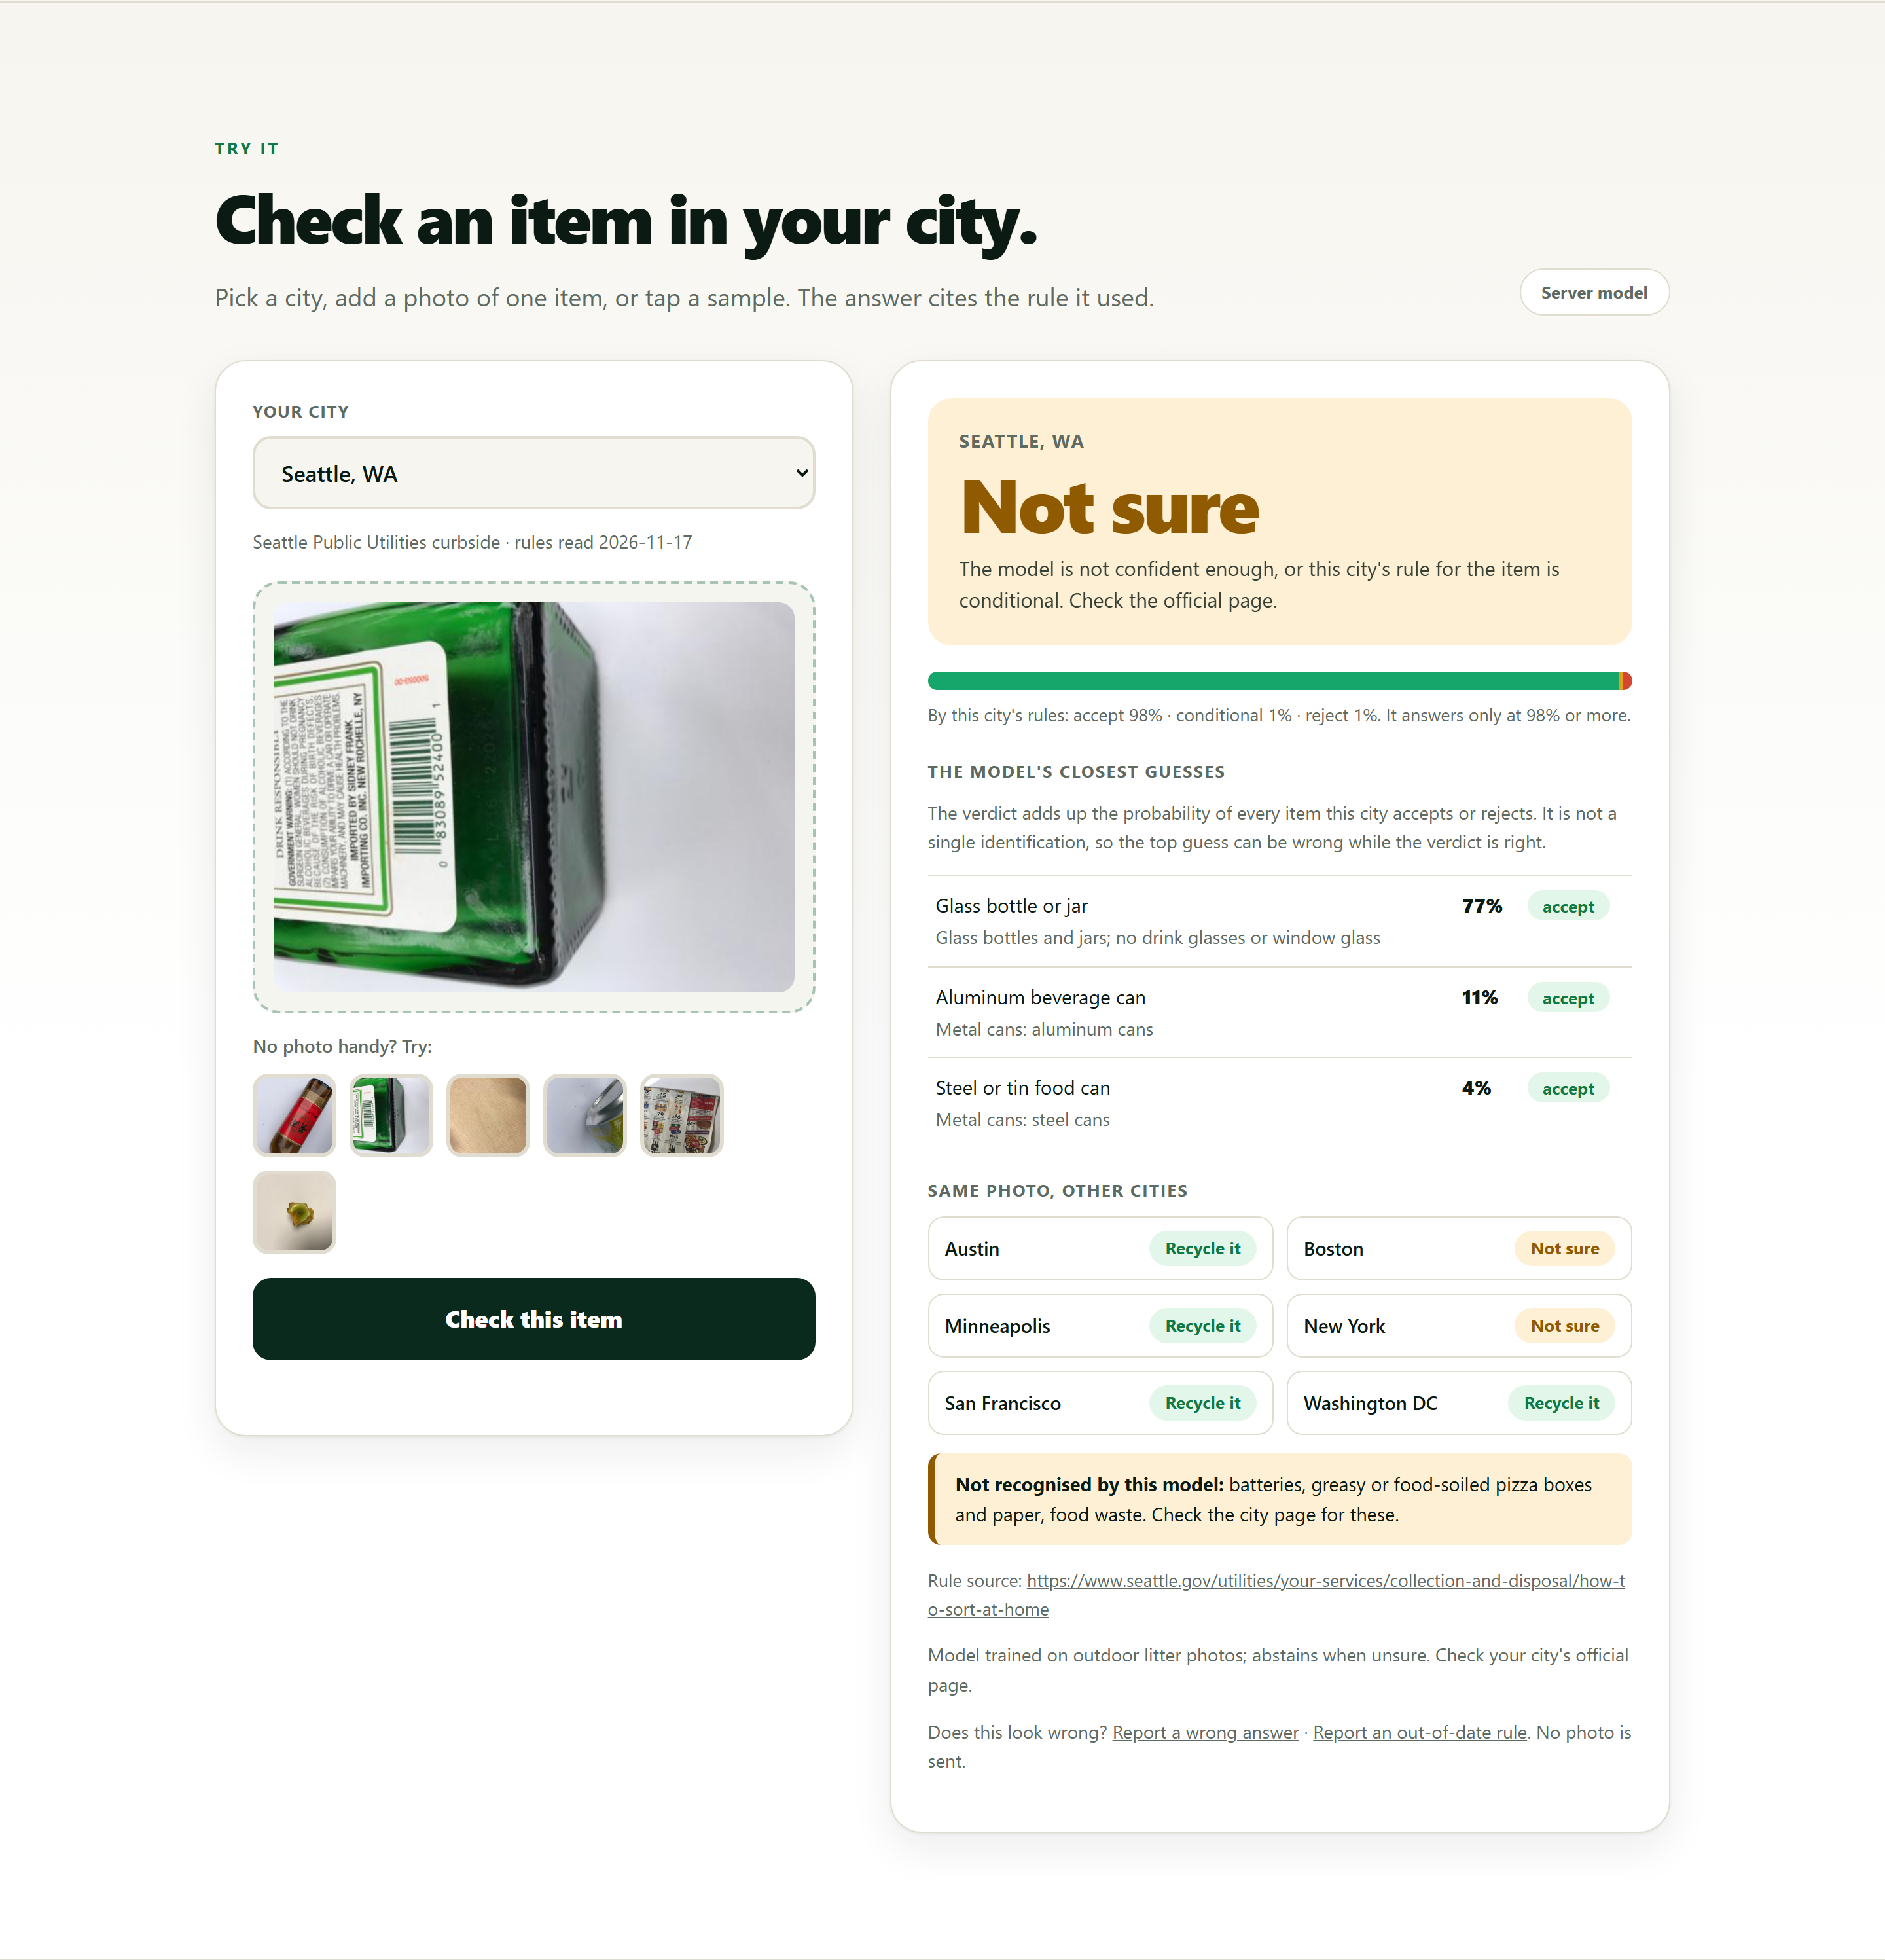
\includegraphics[width=.48\linewidth]{../img/05-glass-seattle.png}\hfill
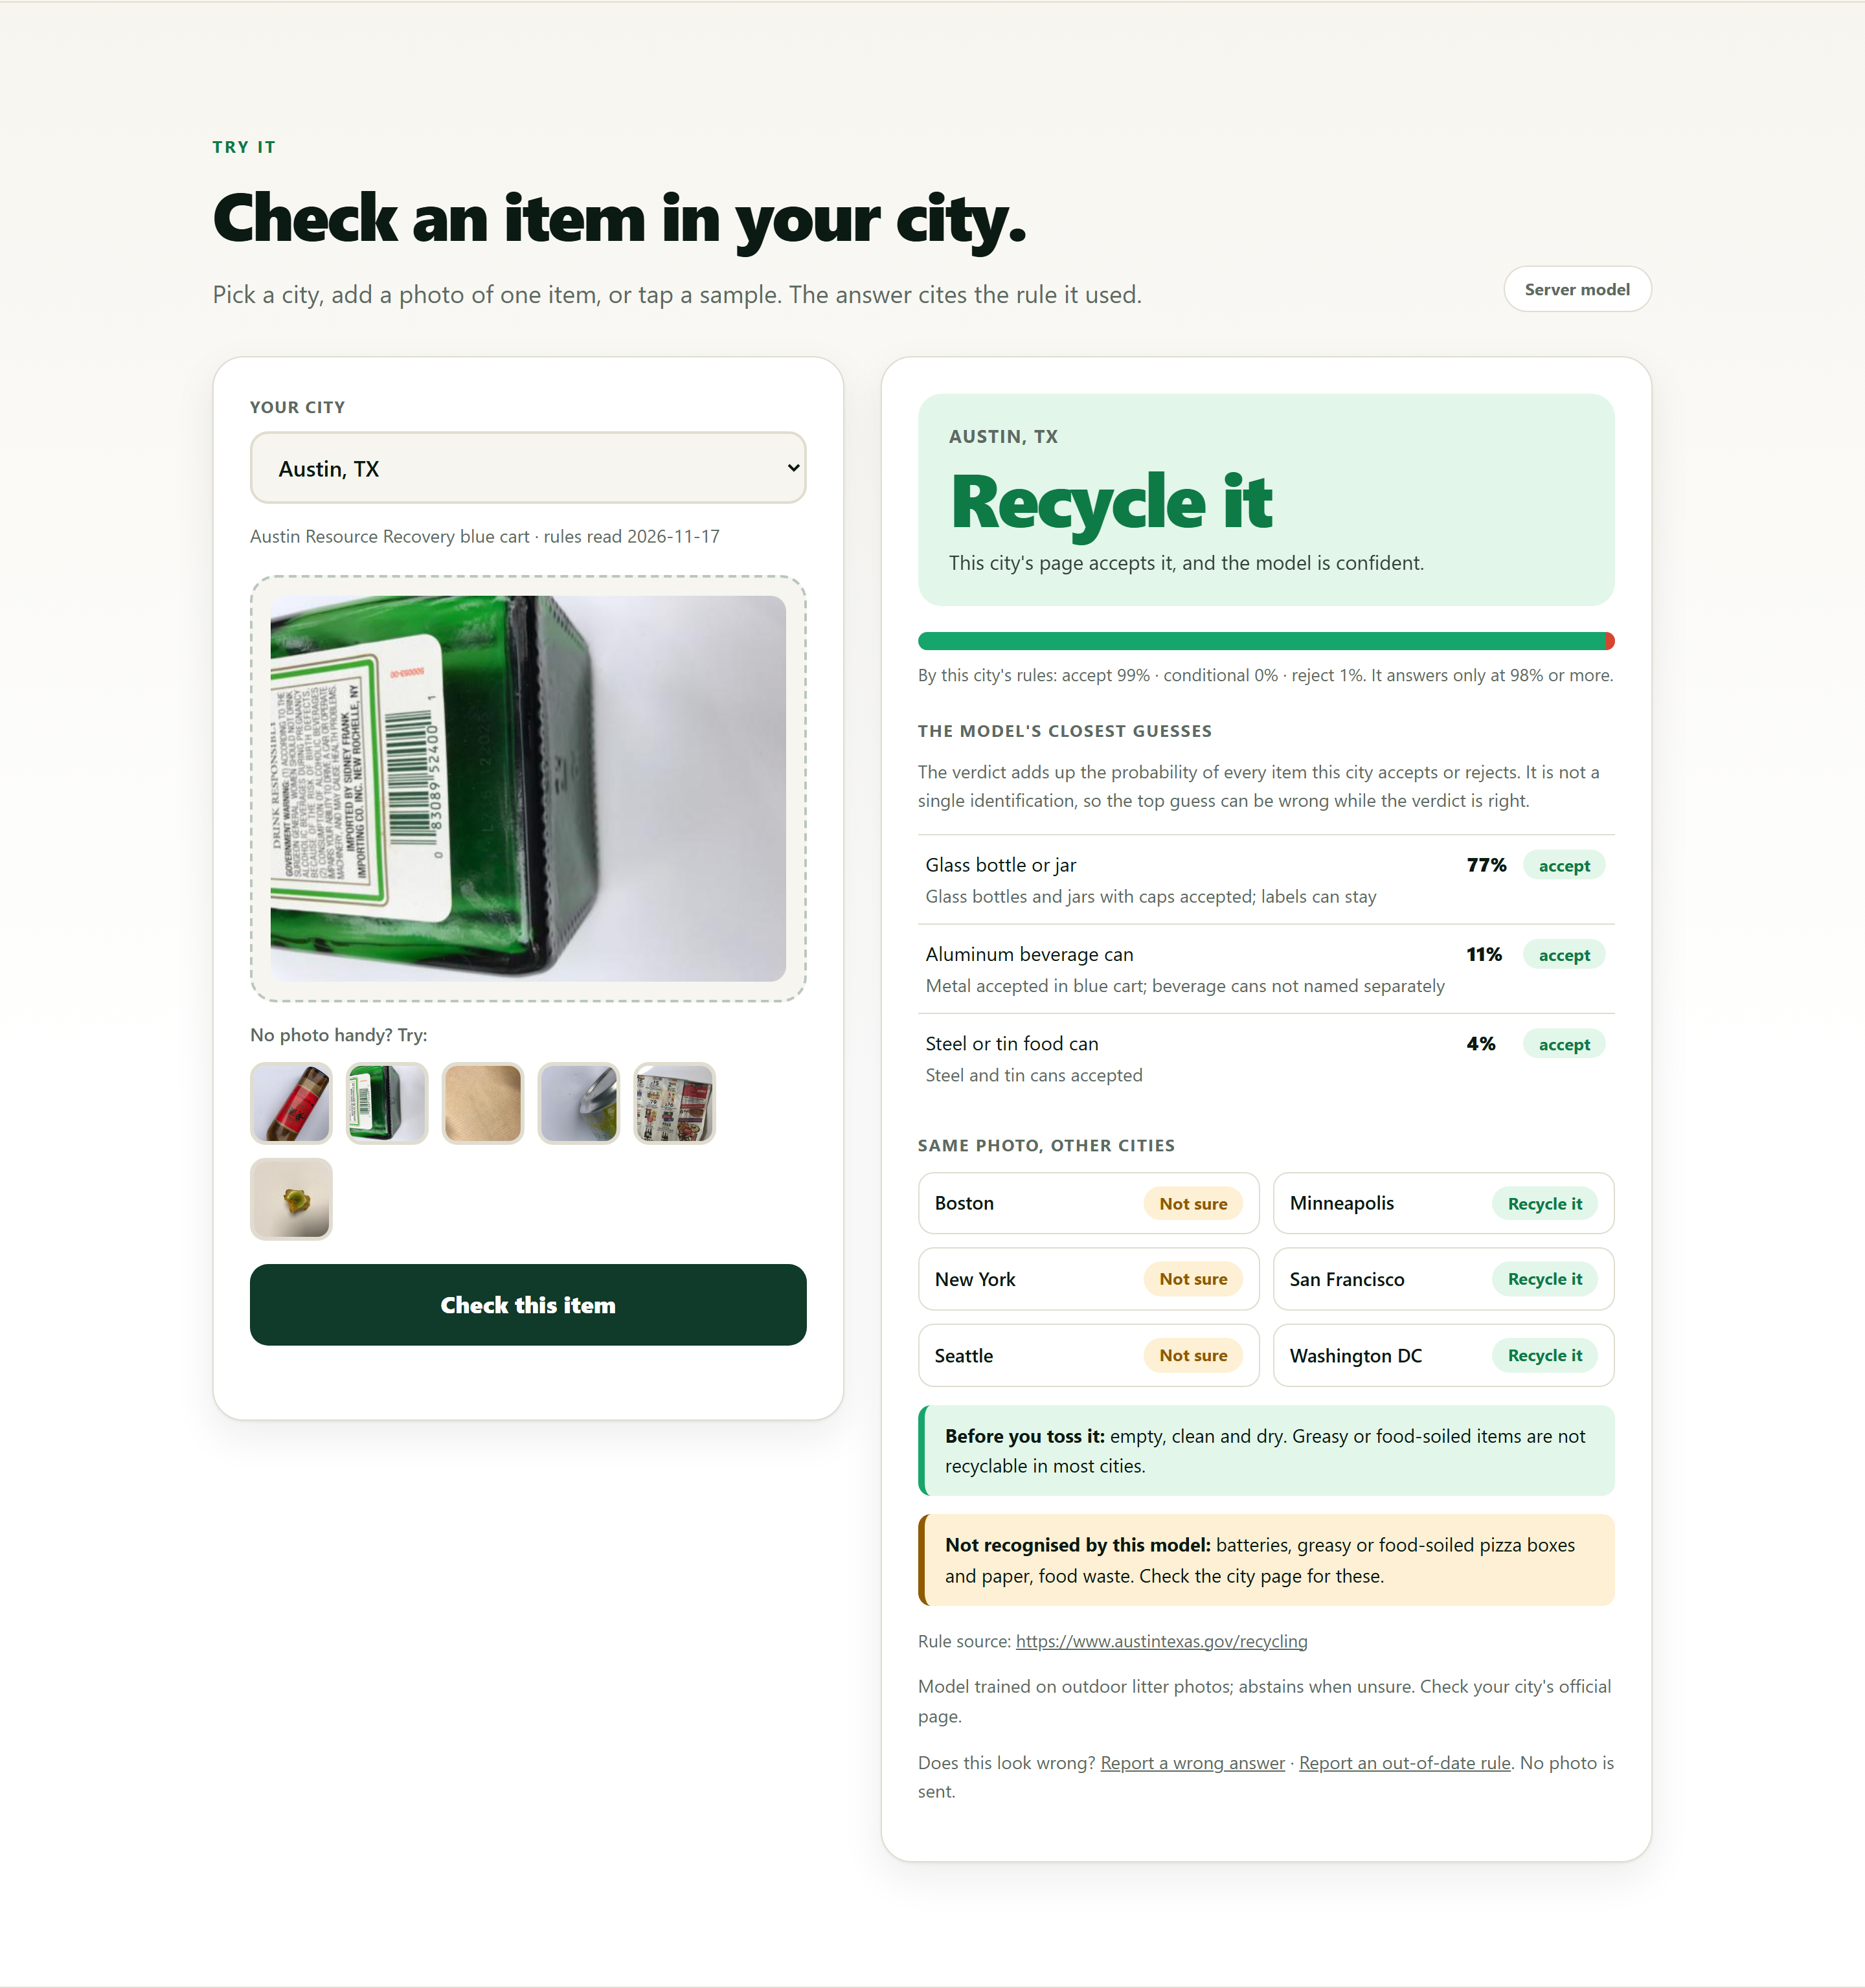
\includegraphics[width=.48\linewidth]{../img/06-glass-austin.png}
\caption{The same glass photo in Seattle (``not sure'': the model is split between items Seattle treats differently) and Austin (``recycle it''). Screenshots of the running application.}\label{fig:ui}
\end{figure}

\section{Data and protocol}
TACO (1{,}563 usable crops after dropping classes under 25 examples and 330 annotations with orientation mismatch) is split by
source photo into train, validation and test (306 test crops). TrashNet (MIT licence) and RealWaste are used both for training and, in leave-one-dataset-out runs, as unseen tests: the model is trained without that dataset and scored on all its non-plastic photos with material-level truth (cardboard, glass, metal, paper count as accept; trash, vegetation, textile and similar count as non-accept; plastic is excluded because its verdict depends on the item). A \emph{false accept} is an accept when the city's rule for the true item is not accept;
a \emph{missed recyclable} is a reject for an accepted item. Dataset licences and unresolved conflicts are in \texttt{docs/DATA.md}.

\section{Results}
\begin{table}[ht]
\centering
\caption{Unseen datasets, Seattle (leave-one-dataset-out; \texttt{eval/v3.json}). Operating point tuned after seeing these tests.}
\begin{tabular}{llrrrr}
\toprule
Test set & Model & False accept & Forced & Missed recyclable & Answered\\
\midrule
TrashNet & shipped & 2.9\% & 61.3\% & 0.00\% & 65.5\%\\
TrashNet & TACO-only & 3.6\% & & 8.1\% & 65.4\%\\
RealWaste & shipped & 2.7\% & 35.4\% & 0.00\% & 29.7\%\\
RealWaste & TACO-only & 1.1\% & & 29.7\% & 69.8\%\\
\bottomrule
\end{tabular}
\end{table}

On the held-out TACO test (Seattle) the earlier model cut false accepts from 15.8\% to 3.3\% at 69\% coverage; the shipped model answers only 19.6\% of those litter crops (0.0\% false accepts).
The browser model is slightly worse on TrashNet (4.4\% to 10.9\% false accepts across cities). Median speed is 166 ms per photo in PyTorch on a laptop CPU and 0.6 s in the browser.

\paragraph{What did not work.} We expected abstaining on city-verdict mass to beat abstaining on item confidence. The two
performed about the same with the trained head and the verdict method was worse with zero-shot features (Figure~\ref{fig:curve}).

\paragraph{Models that looked better and were not.} Adding RealWaste labels alone (v2) cut missed recyclables on held-out RealWaste photos from 30.9\% to 2.2\%, but on unseen TrashNet it wrongly accepted 14\% to 19\%. Training on all three datasets at the original answer target cut missed recyclables to about 0\% but raised false accepts to 9\% to 17\%; a stricter target with the zero-shot blend gave the shipped model, at the cost of answering far less often.

\begin{figure}[ht]
\centering
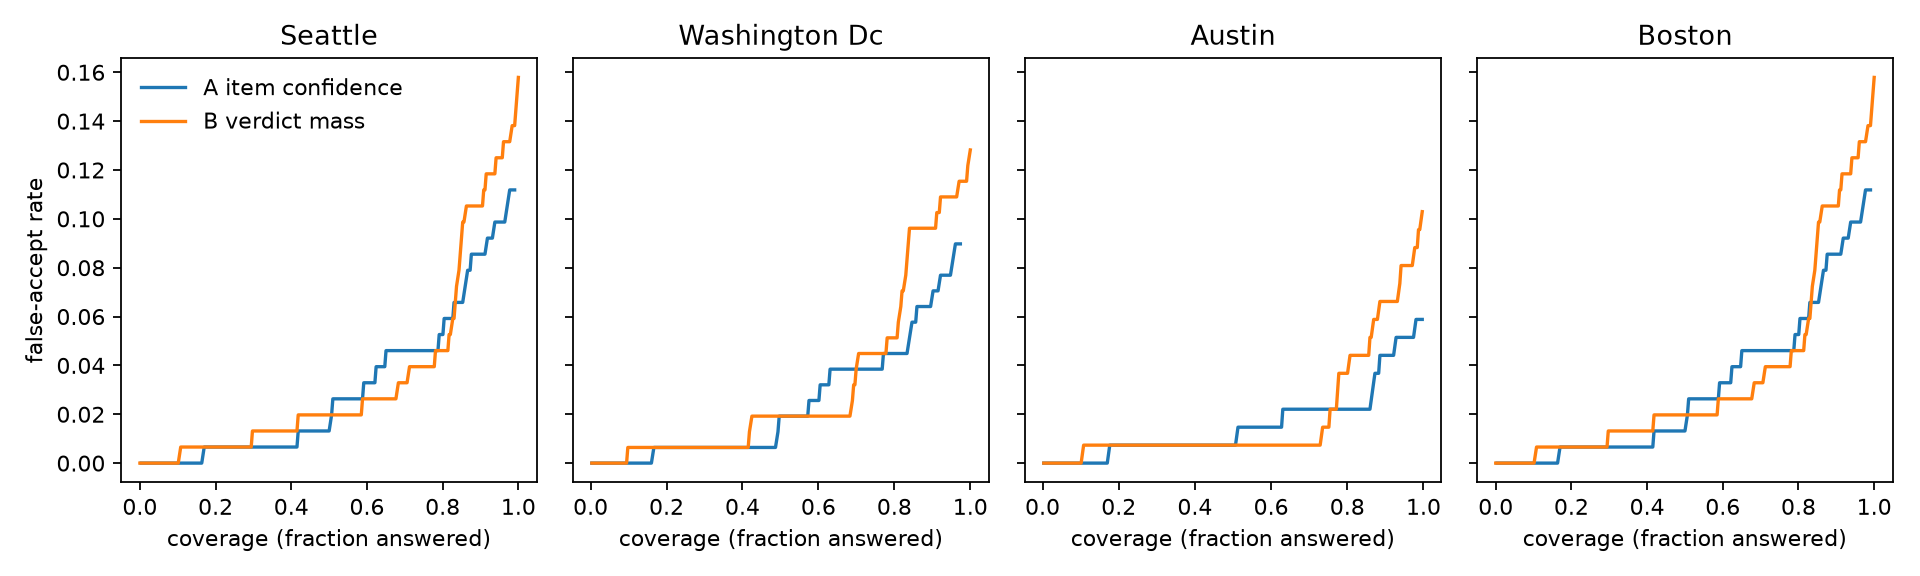
\includegraphics[width=.8\linewidth]{../../eval/far_vs_coverage.png}
\caption{False-accept rate versus coverage on TACO test for item-confidence abstention (A) and verdict-mass abstention (B).}\label{fig:curve}
\end{figure}

\section{Limitations}
Test sets are small and intervals wide. Training data is outdoor litter and landfill photos, not household items.
Batteries, greasy pizza boxes and food waste had too few examples to learn, so the model cannot recognise them; the interface says so on every answer. Seven cities only; where a city page is silent we say
``conditional'', which reflects the page and not necessarily the city's actual rule. Labels for the second dataset are weak
and material-level. The shipped model avoids missed recyclables largely by saying ``not sure'' often; greasy pizza boxes can pass as clean cardboard. No real-world contamination reduction
was measured and none is claimed.

\section{Next steps}
Collect item-level labelled household photos; add machine-readable rules for more cities; evaluate on a fully held-out household
set; pilot with a municipality or sorting facility before making any impact claim.

\section*{Reproducibility}
Code, scripts, evaluation outputs (\texttt{eval/*.json}) and instructions: see the repository README.
\end{document}
